\chapter{Sperimentazione e Risultati}
\label{risultati}

\section{Setup sperimentale}
I test sono stati condotti su una NVIDIA Tesla K80.


\subsection{Partizione in train, test, validation}

Sia per KU-PCP che per LODB, costruiamo le partizioni di training e test destinando a quest'ultima il 20\% delle immagini appartenenti a ciascuna classe e il rimanente 80\% alla partizione di training. Scegliamo questo approccio perchè le suddivisioni già fornite dagli autori dei paper che hanno introdotto i due dataset risultano essere troppo fortemente sbilanciate da poter dividere ulteriormente per ottenere il validation set (vedi Tabella \ref{tab:kupcp_comp}). 

Avendo dataset di dimensioni ridotte, per creare la partizione di validation si opta per la tecnica del \textit{k-fold cross validation}: si suddivide la partizione di training in \(k\) insiemi e si addestra il modello \(k\) volte, ogni volta usando uno dei \(k\) sottoinsiemi come set di test e i restanti \(k-1\) come set di training. Si valutano le performance del modello su ciascun fold e i risultati finali sono la media delle metriche per fold. Scegliamo di utilizzare \(k=5\). I \(k\) insiemi vengono creati casualmente a partire dalla partizione di training.

Tutti i test per la scelta di quale sia la configurazione migliore di layers, learning rates, batch size, epoche da utilizzare vengono fatti sul validation set. I parametri che producono i risultati migliori verranno usati per produrre i risultati definitivi sulla partizione di test.

\subsection{Metriche}

Le metriche utilizzate durante la fase di sperimentazione sono le seguenti: \textit{accuracy} (all), \textit{accuracy} (any), \textit{precision}, \textit{recall}, mAP (\textit{mean average precision}), \textit{F1-score}.

Essendo quello della classificazione della composizione un task multi-label, possiamo decidere di calcolare la accuracy del modello in due modalità, che denominiamo \textit{all} e \textit{any}:
\begin{itemize}
    \item All: una predizione viene considerata corretta solamente quando il modello predice correttamente tutte le classi di ground truth associate a una immagine. Individuare correttamente una su due classificazioni per una stessa immagine conta come zero predizioni corrette. Viene calcolata come il rapporto fra il numero immagini le cui classi sono state tutte predette correttamente e il numero totale di immagini nella partizione di test (o validation).
    \item Any: ogni predizione viene considerata separatamente dalle altre riferite alla stessa immagine. Viene calcolata come il rapporto fra il numero di singole predizioni corrette e il numero di etichette totali nella partizione di test (o validation).
\end{itemize}
Precision e recall vengono calcolate per ciascuna classe:
\begin{itemize}
    \item Precision: il numero di esempi positivi correttamente classificati in una classe sul totale di esempi classificati positivamente per la stessa classe.
    \begin{equation}
        Precision = \frac{TP}{TP + FP}
    \end{equation}
    \item Recall: il numero di esempi positivi correttamente classificati in una classe sul numero di realmente positivi nella stessa classe.
    \begin{equation}
        Recall = \frac{TP}{TP + FN}
    \end{equation}
\end{itemize}
dove:
\begin{itemize}
    \item TP = true positive
    \item FP = false positive
    \item TN = true negative
    \item FN = false negative
\end{itemize}
Troviamo poi la \textit{mean precision} (MP) come media delle precision per classe calcolate in ciascun fold. Introduciamo anche l'F1-score come media armonica di precision e recall per classe:
\begin{equation}
    F1 = 2 \cdot \frac{precision \cdot recall}{precision + recall}
\end{equation}
Il mean F1-score (MF1) è la media degli score delle classi in un fold. 

Il modello deve essere in grado di predirre più di una label per immagine. Per questo motivo, non possiamo scegliere solamente la classe con la probabilità più alta nel vettore di output della rete e considerare quella come unica predizione effettuata dal modello. È necessario porre un \textbf{valore di soglia} sulle probabilità per classe, in modo tale che il vettore delle predizioni possa essere binarizzato: tutte le probabilità al di sopra della soglia sono da considerarsi come classi predette dal modello, mentre quelle al di sotto della soglia saranno ignorate. Le metriche presentate finora verranno calcolate con un valore di threshold \textbf{posto a 0.5}: le classi che hanno una probabilità maggiore del 50\% di essere vere vengono considerate come predizioni del modello.

In questo contesto, introduciamo la \textit{mean average precision} (mAP). La \textit{average precision} (AP) viene definita come l'area sottesa dalla \textit{curva precision-recall}, che viene ottenuta facendo variare il valore di threshold in un determinato intervallo o insieme di valori e disegnando sul grafico i punti corrispondenti ai valori di recall (asse \(x\)) e precision (asse \(y\)) ottenuti a ciascuna soglia, con riferimento ad una classe. Può essere riassunta come:
\begin{equation}
    AP = \sum_n(R_n-R_{n-1})P_n
\end{equation}
dove \(P_n\) e \(R_n\) sono le precision e recall calcolate all'\(n\)-esimo threshold. I valori in cui il threshold varia sono le attivazioni uniche nel vettore di predizioni. La mAP corrisponde alla media delle AP per tutte le classi. Questa metrica è stata definita seguendo l'implementazione della libreria di machine learning per Python \textit{scikit-learn} \cite{sklearn}.

\section{Considerazioni sulle features}
Si presenta uno studio sulla scelta delle features migliori fra quelle esposte nel Capitolo \ref{metodo}, con riferimento al dataset LODB e sulla partizione di validation. Le stesse considerazioni valgono anche per KU-PCP. I risultati finali in test e su entrambi i datasets verranno esplorati nella prossima sezione.

Tutti gli esperimenti in questa fase di considerazioni vengono eseguiti con la seguente configurazione:
\begin{itemize}
    \item Batch size: 1024
    \item Loss: BCE with logits
    \item Epoche: 100
    \item Encoder: ViT-S/14
    \item Optimizer: SDG (\textit{stochastic gradient descent})
    \item Features di DINOv2 in input a un layer lineare
\end{itemize}
Le epoche vengono mantenute fisse e viene modificato solamente il \textit{learning rate}, per poter avere un confronto più equo fra le varie configurazioni. Si scelgono 100 epoche perché costituiscono un numero abbastanza alto di iterazioni da permettere un allenamento che metta in risalto le differenze fra le varie configurazioni, ma abbastanza basso da poter di lanciare più test in maniera sufficientemente rapida. Aumentando il numero di epoche di training i modelli possono migliorare le loro prestazioni, ma in fase di validation l'obiettivo è quello di trovare la combinazione di parametri migliori ai fini del testing finale, non quella di produrre già il risultato migliore possibile.

\subsection{CLS}
Si effettua un confronto fra l'utilizzo del token [CLS] dell'ultimo transformer block contro l'estrazione di più tokens da più blocchi. Si osserva che i risultati migliori in accuracy (any) sono ottenuti utilizzando un solo token [CLS], Tabella \ref{tab:cls_prove}. 

Osserviamo che aumentando il numero di layer considerati, le accuracy tendono a a calare sempre di più. Potremmo attribuire questo fenomeno al fatto che sia altamente probabile che le \textbf{features di DINOv2 non si adattino al task di classificazione della composizione}, per la modalità in cui il modello è pre-allenato e allo scopo per cui viene allenato, la classificazione semantica. Aumentare il numero di features aggiunge informazioni irrilevanti, che non fanno altro che inquinare le predizioni del modello e aumentarne la difficoltà nel convergere, portando a risultati pessimi. Questo spiegherebbe anche perché, pure utilizzando un solo token, le prestazioni su molte classi che rappresentano concetti più astratti e meno semanticamente significativi, come \textit{O2Hor}, \textit{DiaL.}, rispetto a classi come \textit{Pattern}, \textit{Triangle}, \textit{Hor}, siano scarse. Questo aspetto verrà meglio esplorato nel prossimo capitolo (Sezione \ref{dinov2_conclusioni}).

Inoltre, lo sbilanciamento del dataset LODB influisce fortemente sulla natura dei risultati. Il modello tende a predirre più frequentemente le classi di cui ha tanti esempi, come \textit{Center}, \textit{DiaX}, \textit{Hor.} (vedi Tabella \ref{tab:lodb_comp}), e a predirre raramente (o mai) classi poco frequenti, come \textit{O2DiaL.} e \textit{O3Tri.}. Questo si nota dalle matrici di confusione per classe (Tabella \ref{tab:conf_mat}) e dal confronto fra precision e recall (Tabella \ref{tab:cls_precision_recall}): alcune classi hanno una alta precision perchè il modello le predice solamente nei rari casi in cui è sicuro che siano corrette, probabilmente perchè molto simili ai pochi esempi che ha visto in training, ma hanno recall molto bassa perchè le predizioni del modello sono sempre orientate verso le classi di cui ha tanti esempi e meno verso classi meno frequenti. Del totale delle istanze di una determinata classe, ne vengono individuate solamente una porzione molto ridotta. Questo fenomeno è riassunto anche dagli F1-scores, alti solo in corrispondenza di classi numerose. Esistono comunque delle eccezioni. Ad esempio, \textit{Pattern} viene riconosciuto in buona parte dei casi, nonostante abbia un numero ridotto di immagini nel dataset, probabilmente perché rappresenta un concetto molto diverso da tutte le altre classi, che lo rende più facilmente riconoscibile e meno confondibile.


%Da solo
\vspace{5mm}
\begin{table}[h]
    \centering
    \setlength{\tabcolsep}{5pt} % horizontal padding
    \renewcommand{\arraystretch}{1.6} %height
    \begin{tabular}{c|c|ccccc}
        \hline
         Features & lr & & \textbf{Acc. (Any)} & \textbf{Acc. (All)} & \textbf{MP} & \textbf{mAP} \\
         \hline
         CLS$_{12}$ & 0.05 & & \textbf{0.52} & 0.42 & 0.46 & 0.49 \\
         CLS$_{9}$ ... CLS$_{12}$ & 0.006 & & 0.45 & 0.44 & 0.65 & 0.58 \\
         CLS$_{5}$ ... CLS$_{12}$ & 0.002 & & 0.38 & 0.37 & 0.58 & 0.56 \\
         CLS$_{1}$ ... CLS$_{12}$ & 0.0005 & & 0.20 & 0.19 & 0.33 & 0.47 \\
         \hline
    \end{tabular}
    \caption{Un confronto fra le prestazioni del layer lineare utilizzando diverse combinazioni di layer di token [CLS]}
    \label{tab:cls_prove}
\end{table}

\begin{table}[p]
    \centering
    \setlength{\tabcolsep}{5pt} % horizontal padding
    \renewcommand{\arraystretch}{1.6} %height
    \begin{tabular}{c|c|c|c}
         Classe & \textbf{Precision} & \textbf{Recall} & \textbf{F1-score} \\
         \hline
         \hline
\textit{DiaL.}      &                0.8235   &    0.1818   &    0.2979   \\ 
\textit{O2DiaR.}    &                0.2500   &    0.0208   &    \textbf{0.0385}   \\ 
\textit{O2Hor.}     &                0.8000   &    0.1176   &    0.2051   \\ 
\textit{Hor.}       &                0.9080   &    0.8495   &    0.8778   \\ 
\textit{Cent.}      &                0.7079   &    0.5164   &    0.5972   \\ 
\textit{Pat.}       &                0.9730   &    0.7059   &    0.8182   \\ 
\textit{Radi.}      &                0.0000   &    0.0000   &    \textbf{0.0000}   \\ 
\textit{RoT.R}      &                0.7000   &    0.1795   &    0.2857   \\ 
\textit{Ver.}       &                0.9273   &    0.6623   &    0.7727   \\   
\textit{O3Li.}      &                0.5000   &    0.0400   &    \textbf{0.0741}   \\ 
\textit{RoT.L}      &                0.5000   &    0.0303   &    \textbf{0.0571}   \\
\textit{DiaR.}      &                0.8182   &    0.2500   &    0.3830   \\
\textit{DiaX.}      &                0.8952   &    0.8538   &    0.8740   \\
\textit{O3Tri.}     &                0.0000   &    0.0000   &    \textbf{0.0000}   \\
\textit{O2DiaL.}    &                0.0000   &    0.0000   &    \textbf{0.0000}   \\
\textit{Oline}      &                1.0000   &    0.1818   &    0.3077   \\
\textit{Tri.}       &                0.8529   &    0.4915   &    0.6237   \\
    \end{tabular}
    \caption{Metriche per classe del quinto fold nella configurazione CLS$_5$ ... CLS$_{12}$ (8 layers), lr = 0.002. Si nota come gli F1-scores più alti siano in corrispondenza delle classi più numerose nel dataset. Allo stesso modo, le classi che hanno alta precision e bassa recall sono quelle meno frequenti o più granulari, che spesso codificano differenze nel numero dei soggetti nell'immagine. }
    \label{tab:cls_precision_recall}
\end{table}

\begin{table}[p]
    \centering
    \setlength{\tabcolsep}{5pt} % horizontal padding
    \renewcommand{\arraystretch}{1.6} %height
    
    \begin{minipage}{0.4\linewidth}
        \centering
        \raggedright
        \begin{tabular}{c|c|c}
                  & $\sim$ \textit{DiaX} & \textit{DiaX} \\
            \hline
            $\sim$ \textit{DiaX} &  805  & \textbf{13} \\
            \hline
            \textit{DiaX} &  19   & \textbf{111} \\
        \end{tabular}
    \end{minipage}%
    \begin{minipage}{0.4\linewidth}
        \centering
        \raggedleft
        \begin{tabular}{c|c|c}
              & $\sim$ \textit{O3Tri} & \textit{O3Tri} \\
        \hline
        $\sim$ \textit{O3Tri} &  937  & \textbf{0} \\
        \hline
        \textit{O3Tri} &  11   & \textbf{0} \\
    \end{tabular}
    \end{minipage}
        
    
    \caption{Matrici di confusione del quinto fold per \textit{DiaX} e \textit{O3Tri} nella configurazione 8 CLS e lr = 0.002 e nel fold 5. Si nota come \textit{DiaX}, che conta 861 esempi nel dataset, venga individuata correttamente la maggior parte delle volte, mentre \textit{O3Tri}, 115 esempi, non venga mai predetta, da cui le metriche azzerate in Tabella \ref{tab:cls_precision_recall}. Si vede anche come in questo specifico fold siano presenti 130 istanze di \textit{DiaX}, contro solamente 11 di \textit{O3Tri.}}
    \label{tab:conf_mat}
    
\end{table}


\subsection{AVG}
Usare un patch AVG migliora leggermente le prestazioni della rete in confronto ad utilizzare un token CLS, in termini di accuracy e precision (Tabella \ref{tab:avg_prove}). Il sospetto è che CLS sia meno indicato ai fini della classificazione per un task scollegato alla semantica, perchè appreso durante il training di DINO appositamente per racchiudere il significato semantico dell'immagine. Mediare i patch, invece, può fornire informazioni più varie su cui distinguere le diverse classi. In generale, però, anche usando AVG i risultati sono sotto le aspettative e utilizzare più layers porta ad un deterioramento delle prestazioni. Potremmo interpretarlo come ulteriore sintomo del fatto che le features di DINOv2 non siano adatte al task. 

\begin{table}[h]
    \centering
    \setlength{\tabcolsep}{5pt} % horizontal padding
    \renewcommand{\arraystretch}{1.6} %height
    \begin{tabular}{c|c|ccccc}
        \hline
         Features & lr & & \textbf{Acc. (Any)} & \textbf{Acc. (All)} & \textbf{MP} & \textbf{mAP} \\
         \hline
         AVG$_{12}$               & 0.06   & & \textbf{0.52} & \textbf{0.49} & \textbf{0.61} & \textbf{0.59} \\
         AVG$_{9}$ ... AVG$_{12}$ & 0.005  & & 0.43 & 0.42 & 0.60 & 0.59 \\
         AVG$_{5}$ ... AVG$_{12}$ & 0.002  & & 0.41 & 0.41 & 0.55 & 0.56 \\
         AVG$_{1}$ ... AVG$_{12}$ & 0.001 & & 0.35 & 0.34 & 0.51 & 0.54 \\
         \hline
    \end{tabular}
    \caption{Un confronto fra le prestazioni del layer lineare utilizzando diverse combinazioni di layer di AVG patch}
    \label{tab:avg_prove}
\end{table}



\subsection{Concatenazione di CLS e AVG}
Si osserva un leggero miglioramento delle prestazioni utilizzando i due tipi di feature in combinazione (Tabella \ref{tab:cls_avg_prove}). Inoltre, i risultati migliorano aumentando il numero di layers considerati, soprattutto in termini di precision. Potremmo stimare che usare i due token in coppia possa fornire due tipologie di informazione diversa che la rete riesce a sfruttare meglio piuttosto che riceverle singolarmente, ma il guadagno in prestazioni è troppo basso per poter giungere a conclusioni significative. 

Inoltre, si provano anche a combinare primi e ultimi layers di CLS e AVG, per verificare se in questa modalità sia possibile raccogliere informazioni provenienti da diversi livelli di astrazione, come accade nelle CNN, che possano aiutare in un task scollegato dalla semantica come la composizione. Dai risultati ottenuti, però, non possiamo giungere a questa conclusione.
\vspace{5mm}
\begin{table}[h]
    \centering
    \setlength{\tabcolsep}{5pt} % horizontal padding
    \renewcommand{\arraystretch}{1.6} %height
    \begin{tabular}{m{6.25cm}|c|ccccc}
        \hline
         Features & lr & & \textbf{Acc. (Any)} & \textbf{Acc. (All)} & \textbf{MP} & \textbf{mAP} \\
         \hline
         CLS$_{12}$AVG$_{12}$               & 0.01  & & 0.49 & 0.46 & 0.58 & 0.56 \\
         CLS$_{9}$ ... CLS$_{12}$ AVG$_9$ ... AVG$_{12}$ & 0.005  & & \textbf{0.51} & \textbf{0.49} & \textbf{0.64} & \textbf{0.63} \\
         CLS$_{5}$ ... CLS$_{12}$AVG$_{5}$ ... AVG$_{12}$ & 0.001  & & 0.42 & 0.41 & 0.63 & 0.60 \\
         CLS$_{1}$ ... CLS$_{4}$CLS$_{9}$ ... CLS$_{12}$ AVG$_{1}$ ... AVG$_{4}$AVG$_{9}$ ... AVG$_{12}$ & 0.001 && 0.39 & 0.38 & 0.56 & 0.58 \\
         \hline
    \end{tabular}
    \caption{Un confronto fra le prestazioni del layer lineare utilizzando diverse combinazioni di layer di token [CLS] e AVG patch.}
    \label{tab:cls_avg_prove}
\end{table}


\section{Risultati finali}
La configurazione di features scelta è di 4 token [CLS] e 4 AVG patch dei layer finali. Con questa e con batch size 1024, SGD e ViT-S/14 si fanno ulteriori prove in validation per stabilire il numero migliore di epoche e learning rate da usare in fase di test.

Si è sperimentato anche usando ViT-B e ViT-L (Appendice \ref{tipologie_vit}), ma non si sono osservati miglioramenti significativi delle prestazioni del modello, a fronte di una richiesta di risorse di tempo e memoria fisica nettamente aumentate. 

\subsection{Linear layer}

Si riportano i risultati ottenuti su LODB e KUPCP in Tabella \ref{tab:linear_test}. I risultati su LODB non sono direttamente paragonabili a quelli del paper \cite{graph} che lo ha introdotto (discusso in Sezione \ref{graph}) perché le metriche da loro esposte sono legate al metodo da loro utilizzato (graph attention network). Possiamo comunque concludere che le prestazioni siano nettamente al di sotto di quella che potremmo definire una buona prestazione. I risultati su KU-PCP sono migliori, ma ancora inferiori a quelli ottenuti da altri metodi in letteratura (Tabella \ref{tab:kupcp_sota_comparison}). In Tabella \ref{tab:kupcp_metriche_classe} si riportano le metriche per classe per KU-PCP e in Tabella \ref{tab:lodb_metriche_classe} quelle per LODB, nelle Figure \ref{fig:loss-lodb-linear} e \ref{fig:loss-kupcp-linear} i grafici delle loss, che non mostrano segni di overfitting. Dalla Figura \ref{fig:kupcp_prob} si trovano le predizioni effettuate dalla rete per alcune immagini di entrambi i datasets, che mettono in risalto alcune delle loro criticità.

\vspace{5mm}
\begin{table}[h]
    \centering
    \setlength{\tabcolsep}{5pt} % horizontal padding
    \renewcommand{\arraystretch}{1.6} %height
    \begin{tabular}{c|cc|ccccc}
         \hline
         Dataset & Epoche & lr & \textbf{Acc. (Any)} & \textbf{Acc. (All)} & \textbf{MP} & \textbf{mAP} & \textbf{MF1} \\
          \hline
          KUPCP & 300 & 0.003 & 0.83 & 0.63 & 0.84 & 0.81 & 0.79 \\
          LODB & 200 & 0.003 & 0.56 & 0.52 & 0.66 & 0.65 & 0.49 \\
          \hline
    \end{tabular}
    \caption{Risultati in fase di test utilizzando un linear layer. Tutti i risultati sono presentati con threshold per le probabilità posto a 0.5.}
    \label{tab:linear_test}
\end{table}

\vspace{5mm}
\begin{table}[h]
    \centering
    \setlength{\tabcolsep}{5pt} % horizontal padding
    \renewcommand{\arraystretch}{1.6} %height
    \begin{tabular}{l|c}
         \hline
         \textbf{Metodo} & \textbf{Acc. (Any) \%} \\
         \hline
         FT\_CNN \cite{composition_dominant_geometric} &  88.8 \\
         RSTN \cite{spatial_invariant_cnn} & 90.9 \\
         DINOv2 + linear & 82.9 \\
          \hline
    \end{tabular}
    \caption{Confronto fra il nostro metodo e gli altri metodi in letteratura sviluppati per la classificazione su KU-PCP discussi nel Capitolo \ref{sota}.}
    \label{tab:kupcp_sota_comparison}
\end{table}

\begin{table}[p]
    \centering
    \setlength{\tabcolsep}{5pt} % horizontal padding
    \renewcommand{\arraystretch}{1.6} %height
    \begin{tabular}{c|c|c|c}
         Classe & \textbf{Precision} & \textbf{Recall} & \textbf{F1-score} \\
         \hline
         \hline
\textit{DiaL.}               &       0.7333   &    0.3438   &    0.4681       \\
\textit{O2DiaR.}             &      0.2381    &   0.0847    &   \textbf{0.1250}       \\
\textit{O2Hor.}              &       0.4545   &    0.1923   &    \textbf{0.2703}       \\
\textit{Hor.}                &       0.9630   &    0.8254   &    0.8889       \\
\textit{Cent.}               &       0.8129   &    0.7079   &    0.7568       \\
\textit{Pat.}                &       0.9091   &    0.7843   &    0.8421       \\
\textit{Radi.}               &       0.5294   &    0.4286   &    0.4737       \\
\textit{RoT.R}               &       0.8333   &    0.5263   &    0.6452       \\
\textit{Ver.}                &       0.9615   &    0.8242   &    0.8876       \\
\textit{O3Li.}               &       0.4444   &    0.1143   &    \textbf{0.1818}       \\
\textit{RoT.L}               &       0.7333   &    0.2500   &    0.3729       \\
\textit{DiaR.}               &       0.7895   &    0.3261   &    0.4615       \\
\textit{DiaX.}               &       0.9308   &    0.8605   &    0.8943       \\
\textit{O3Tri.}              &       0.3333   &    0.0417   &    \textbf{0.0741}       \\
\textit{O2DiaL.}             &       0.1429   &    0.0159   &    \textbf{0.0286}       \\
\textit{Oline}               &      0.6250    &   0.2174    &   \textbf{0.3226}       \\
\textit{Tri.}                &      0.8182    &   0.7079    &   0.7590       \\
    \end{tabular}
    \caption{Metriche per classe su LODB in test con linear layer. Come già discusso precedentemente, si notano F1-score bassi in classi poco frequenti o che codificano il conteggio dei soggetti, e score più elevati in classi più numerose, accompagnate da alte precision e recall. }
    \label{tab:lodb_metriche_classe}
\end{table}

\begin{figure}[p]
    \centering
    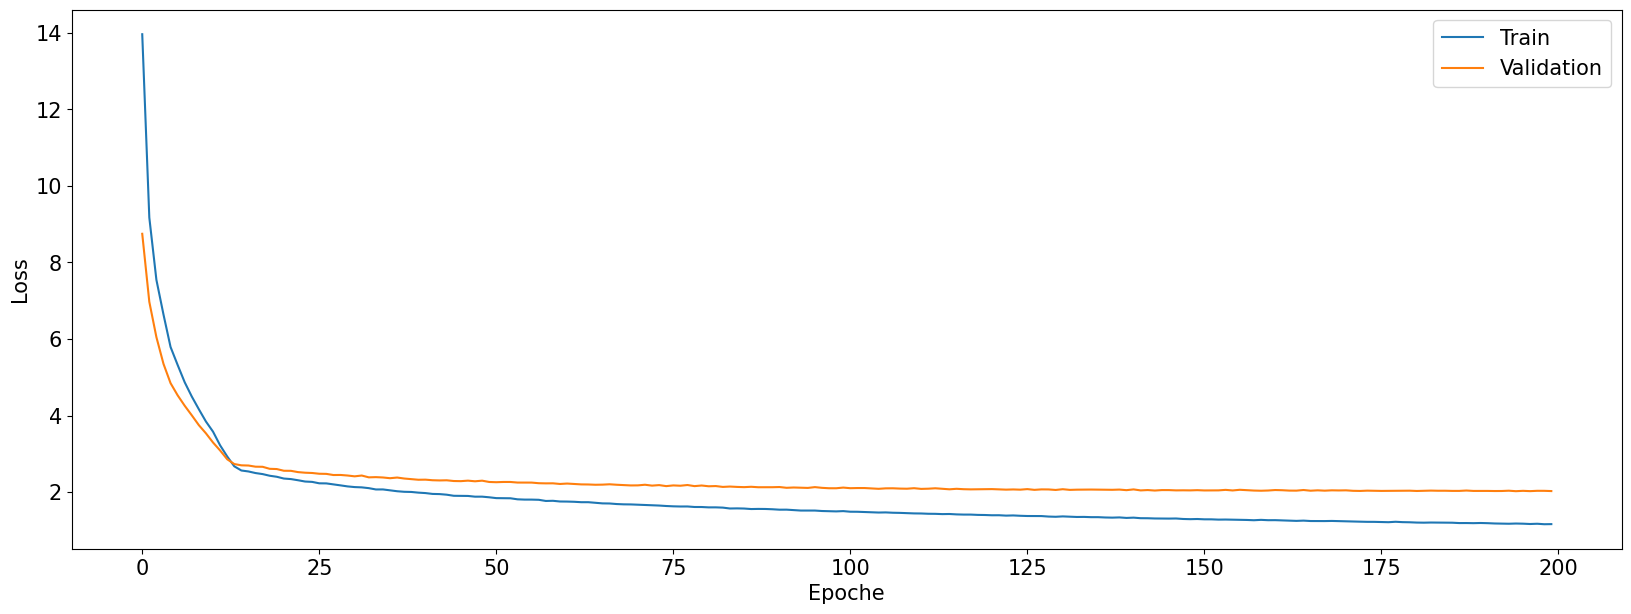
\includegraphics[width=0.8\linewidth]{Immagini/risultati/loss-lodb-linear.png}
    \caption{Grafico della loss in validation (quinto fold) su LODB e linear layer per la configurazione 4 token CLS e 4 AVG patch, 200 epoche, learning rate 0.003, che viene usata in fase di test. Non ci sono segnali di overfitting.}
    \label{fig:loss-lodb-linear}
\end{figure}

\begin{table}[p]
    \centering
    \setlength{\tabcolsep}{5pt} % horizontal padding
    \renewcommand{\arraystretch}{1.6} %height
    \begin{tabular}{c|c|c|c}
         Classe & \textbf{Precision} & \textbf{Recall} & \textbf{F1-score} \\
         \hline
         \hline
\textit{RoT}               &         0.6866    &   0.7480    &   0.7160       \\
\textit{Vertical}          &         0.8571    &   0.6364    &   0.7304       \\
\textit{Horizontal}        &         0.8390    &   0.8190    &   0.8289       \\
\textit{Diagonal}          &         0.7372    &   0.5344    &   0.6196       \\
\textit{Curved}            &         0.7722    &   0.6630    &   0.7135       \\
\textit{Triangle}          &         0.8487    &   0.7544    &   0.7988       \\
\textit{Center}            &         0.9135    &   0.7814    &   0.8423       \\
\textit{Symmetric}         &         0.9770    &   0.8586    &   0.9140       \\
\textit{Pattern}           &         0.9683    &   0.9683    &   0.9683       \\
    \end{tabular}
    \caption{Metriche per classe in test su KU-PCP con linear layer. A supporto della teoria che le features di DINOv2 riconoscano il contenuto semantico nelle immagini e usino quello per la classificazione, come si esplorerà nel prossimo capitolo, \textit{RoT} è la classe con prestazioni peggiori ed è anche quella che presenta varianza semantica intraclasse più elevata, al contrario di classi come \textit{Symmetric} o \textit{Pattern}, che infatti presentano risultati migliori.}
    \label{tab:kupcp_metriche_classe}
\end{table}

\begin{figure}[p]
    \centering
    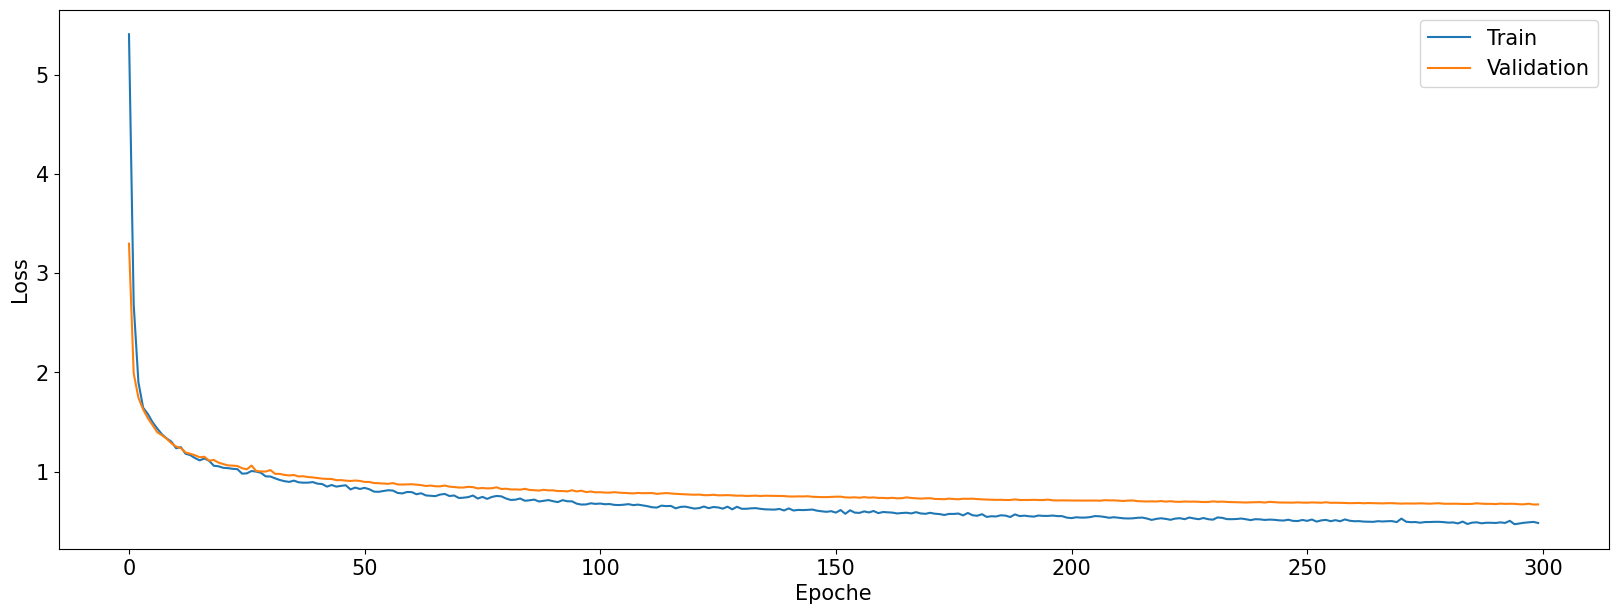
\includegraphics[width=\linewidth]{Immagini/risultati/loss-kupcp-linear.png}
    \caption{Grafico della loss in validation (quinto fold) su KU-PCP e linear layer per la configurazione con 4 token CLS e 4 AVG patch, 300 epoche e learning rate 0.003, che viene usata in fase di test. La discesa della loss non mostra segni di overfitting.}
    \label{fig:loss-kupcp-linear}
\end{figure}

\subsection{MLP}
Con MLP come classificatore, facendo diverse prove e modificando la quantità e tipologia di features usate, su KU-PCP si arriva sempre a pareggiare o stare leggermente al di sotto dei risultati ottenuti tramite layer lineare. Su LODB le differenze sono di poco più pronunciate, ma non si discostano in maniera radicale. Anche le differenze osservate a fronte della scelta di diversi layer di features sono minime. Possiamo affermare che non sia richiesto un modello più complesso di un semplice layer lineare per sfruttare al meglio i dati a disposizione. Come già ribadito, il fattore limitante sono le features, non il classificatore.

Si mantiene la configurazione di 4 token CLS e 4 AVG patch per avere un confronto diretto con i risultati ottenuti tramite layer lineare. I valori finali sono raccolti in Tabella \ref{tab:mlp_test}. Anche le metriche per classe sono pressoché invariate da quelle presentate classificando con linear layer, con differenze non significative nel range 1-2\%, e con le stesse problematiche mostrate su LODB. Per questo motivo non vengono riportate.

\newpage
\begin{table}[p]
    \centering
    \setlength{\tabcolsep}{5pt} % horizontal padding
    \renewcommand{\arraystretch}{1.6} %height
    \begin{tabular}{c|cc|ccccc}
         \hline
         Dataset & Epoche & lr & \textbf{Acc. (Any)} & \textbf{Acc. (All)} & \textbf{MP} & \textbf{mAP} & \textbf{MF1} \\
          \hline
          KUPCP & 200 & 0.005 & 0.84 & 0.54 & 0.83 & 0.76 & 0.77 \\
          LODB & 300 & 0.002 & 0.51 & 0.50 & 0.68 & 0.67 & 0.44 \\
          \hline
    \end{tabular}
    \caption{Risultati in fase di test utilizzando un MLP. I valori sono simili a quelli ottenuti tramite un singolo linear layer (Tabella \ref{tab:linear_test}) con differenze inferiori al 5\% nella maggior parte dei casi, che potrebbero essere ridotte ancora di più prolungando l'allenamento o incrementando il learning rate.}
    \label{tab:mlp_test}
\end{table}

\begin{figure}[p]
    \centering
    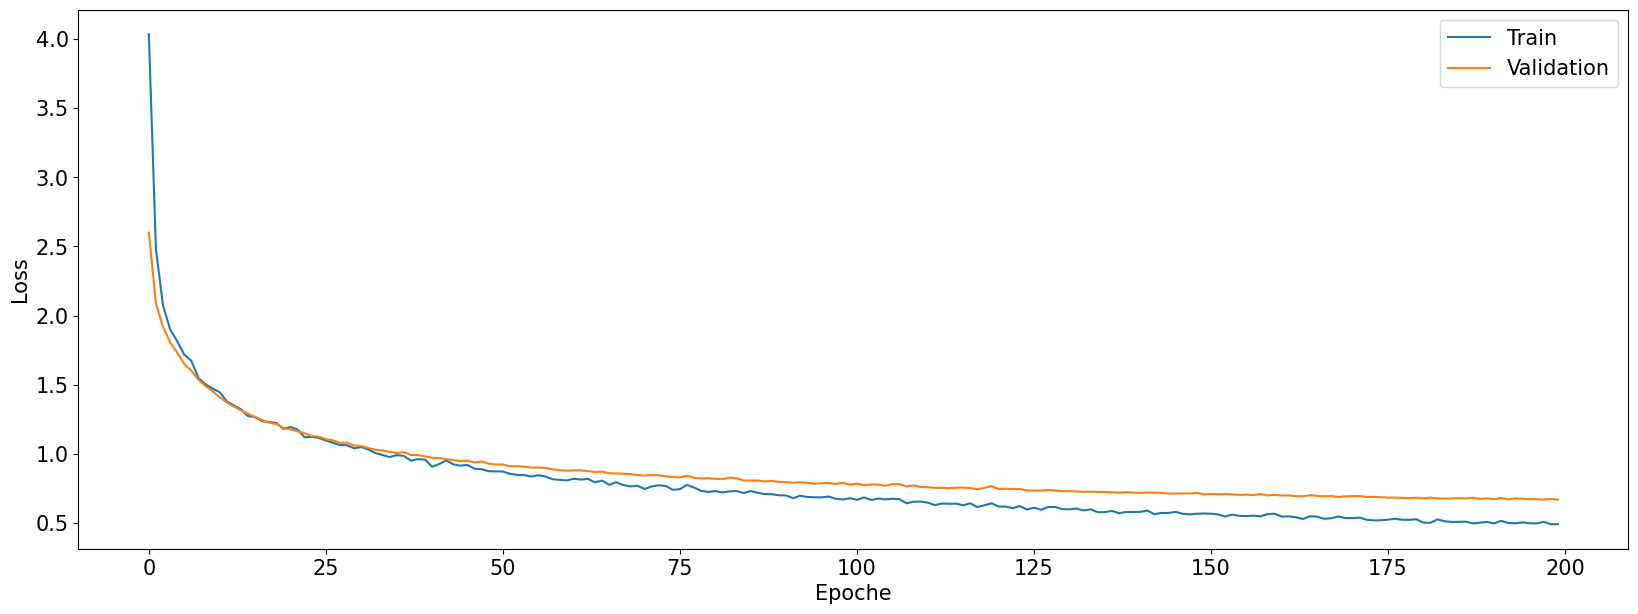
\includegraphics[width=\linewidth]{Immagini/risultati/loss_mlp_kupcp.png}
    \caption{Grafico della loss in validation (quinto fold) su KU-PCP e MLP per la configurazione 4 token CLS e 4 AVG patch, 200 epoche, learning rate 0.005, che viene usata in fase di test. Non ci sono segnali di overfitting.}
    \label{fig:loss-lodb-mlp}
\end{figure}

\begin{figure}[p]
    \centering
    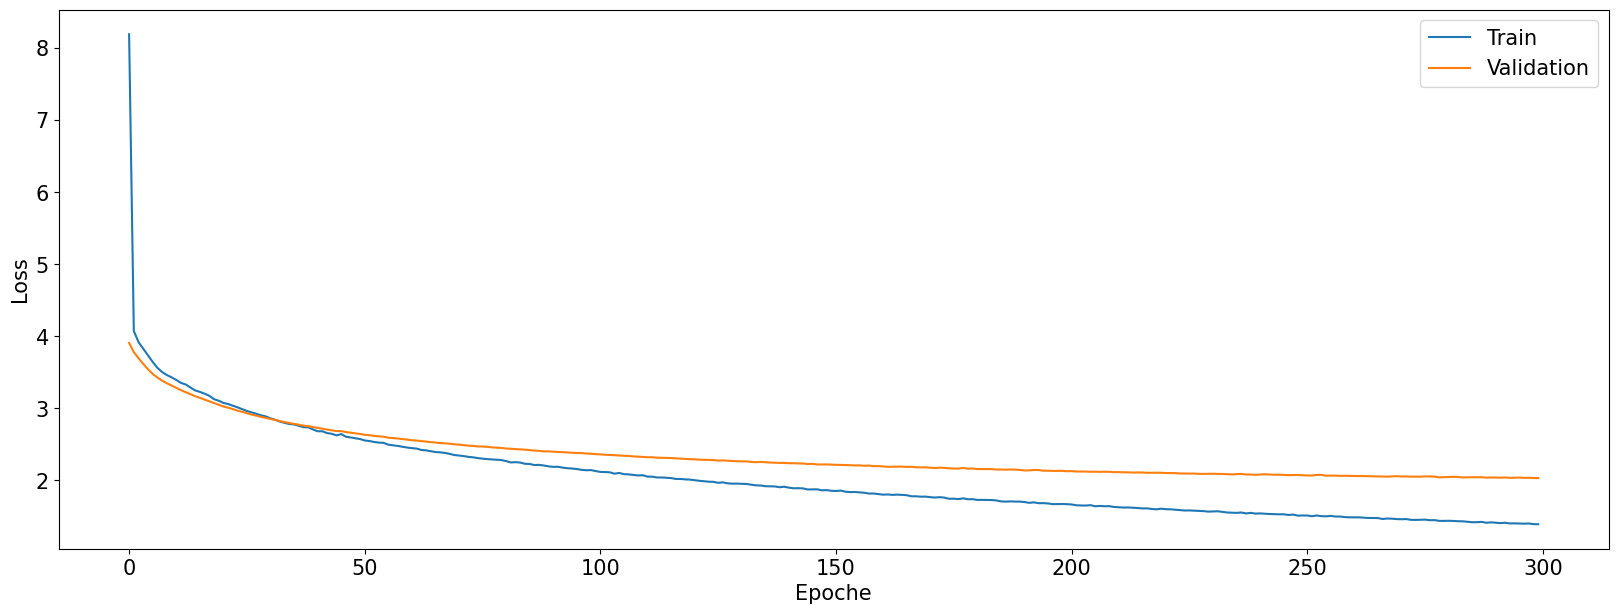
\includegraphics[width=\linewidth]{Immagini/risultati/loss_mlp_lodb.png}
    \caption{Grafico della loss in validation (quinto fold) su LODB e MLP per la configurazione 4 token CLS e 4 AVG patch, 300 epoche, learning rate 0.002, che viene usata in fase di test. Non ci sono segnali di overfitting.}
    \label{fig:loss-lodb-mlp}
\end{figure}



% ALCUNI ESEMPI DI PREDIZIONI CON ISTOGRAMMA
\begin{figure}[p]
    \centering
    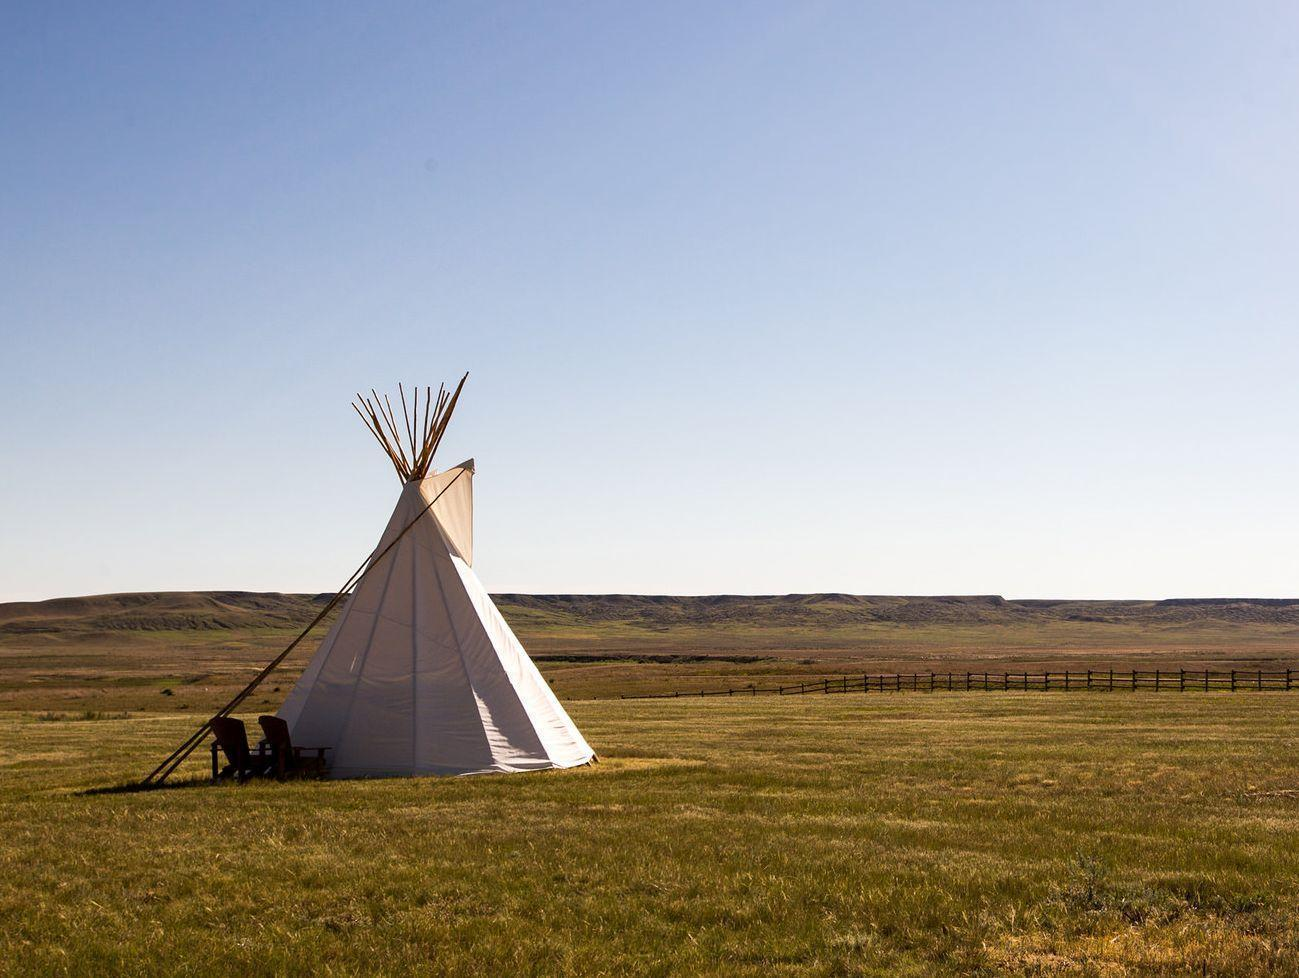
\includegraphics[height=55mm, valign=t]{Immagini/risultati/0207.jpg}
    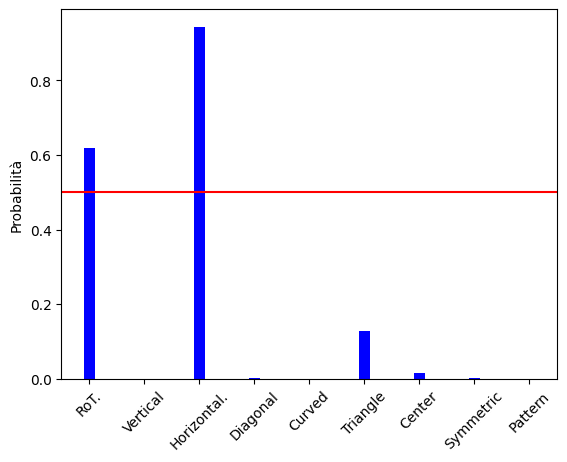
\includegraphics[height=66mm, valign=t]{Immagini/risultati/207_prob.png}
    
    \caption{Esempio di predizione corretta della rete con linear classifier su KU-PCP. Le classi di ground truth sono \textit{RoT.} e \textit{Horizontal}. In rosso è segnata la soglia di threshold (posta a 0.5) utilizzata per il calcolo delle metriche.}
    \label{fig:kupcp_prob}
\end{figure}

\begin{figure}[p]
    \centering
    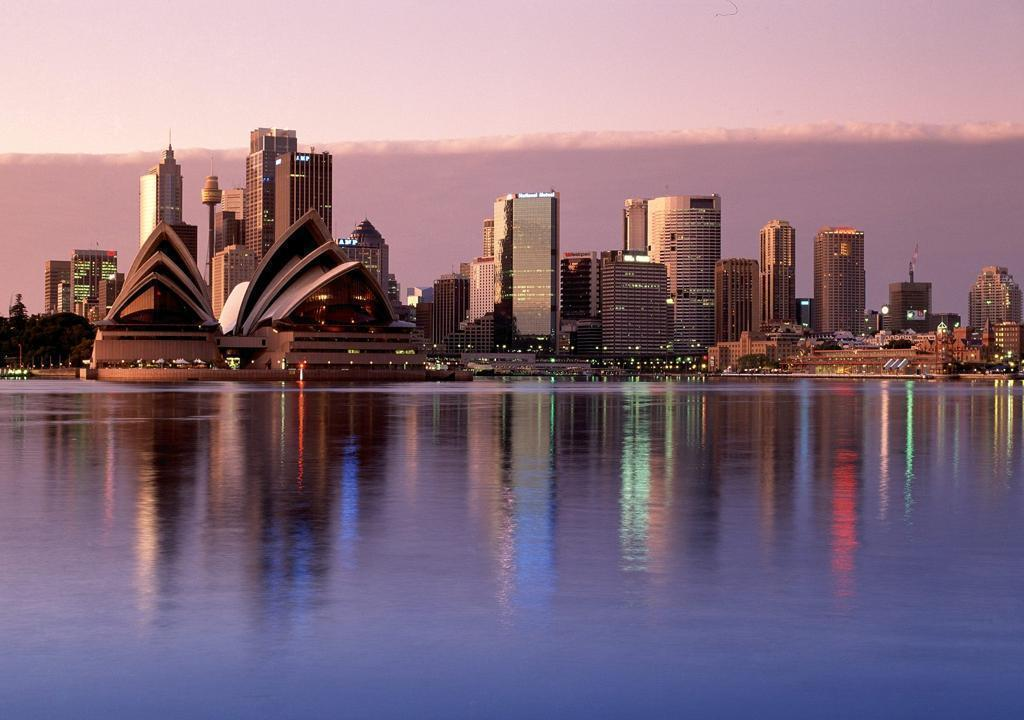
\includegraphics[height=53mm, valign=t]{Immagini/risultati/0626.jpg}
    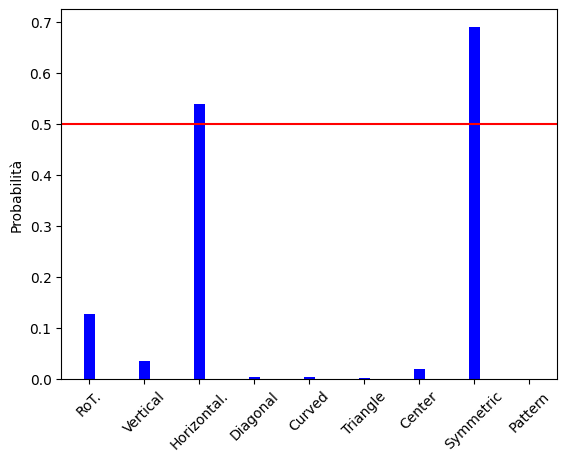
\includegraphics[height=65mm, valign=t]{Immagini/risultati/626_prob.png}
    \caption{Predizione con classificatore lineare su KU-PCP. Le classi di ground truth sono \textit{Vertical} e \textit{Symmetric}, mentre la nostra rete predice \textit{Horizontal} e \textit{Symmetric}. Effettivamente, essendo uno scatto in lontananza della città, somiglia più alle immagini che nel dataset sono classificate come \textit{Horizontal} perchè ritraente un orizzonte, piuttosto che \textit{Vertical}, di cui solitamente fanno parte immagini di palazzi in vista più ravvicinata. Le prestazioni, quindi, sono anche influenzate da un cattivo o non consistente etichettamento delle immagini nel dataset.}
    \label{fig:kupcp_prob2}
\end{figure}


\begin{figure}[p]
    \centering
    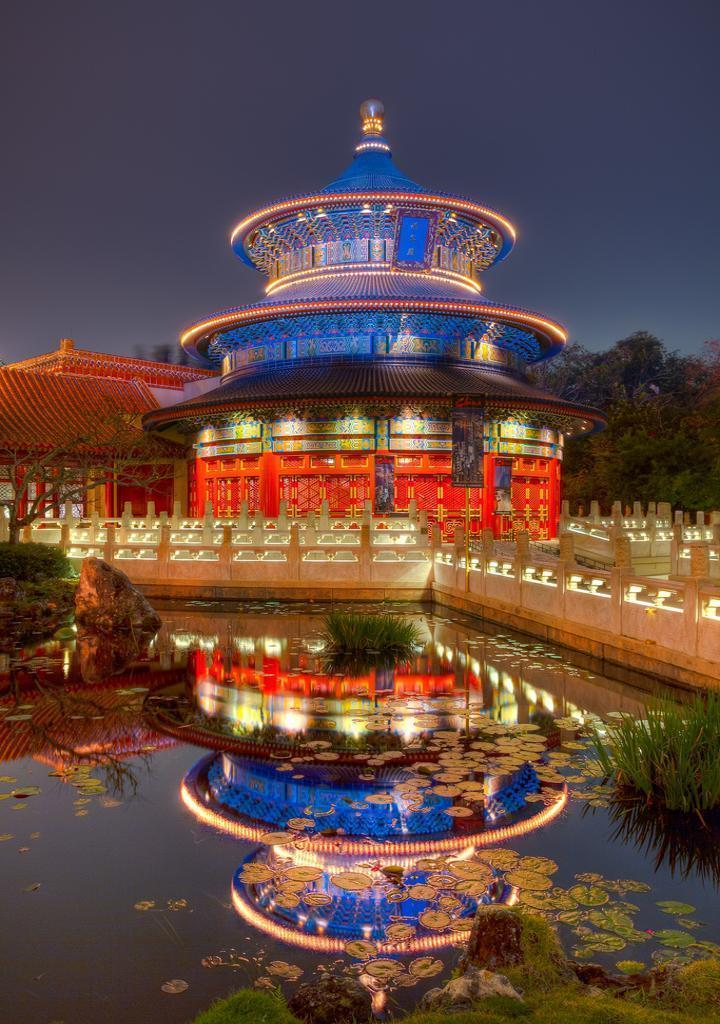
\includegraphics[height=66mm, valign=t]{Immagini/risultati/0730.jpg}
    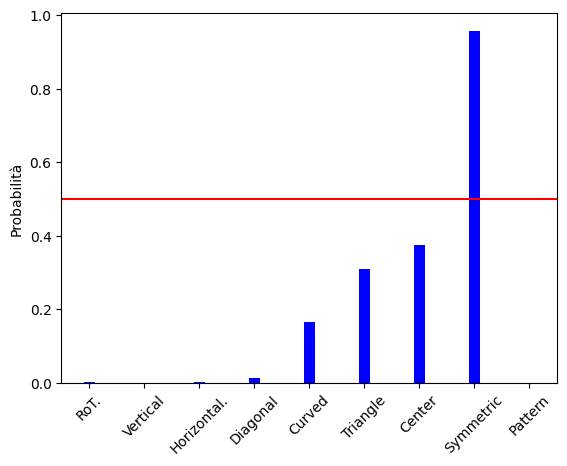
\includegraphics[height=80mm, valign=t]{Immagini/risultati/730_prob.png}
    \caption{Predizione con classificatore lineare su KU-PCP, ground truth \textit{Symmetric} e \textit{Center}. Ancora una volta, l'etichettamento dato all'immagine nel dataset è fuorviante. La rete intuisce la forma dell'edificio e le curve che lo compongono, che sarebbero potute essere altre due valide classi di ground truth per l'immagine in questione.}
    \label{fig:kupcp_prob3}
\end{figure}

\begin{figure}[p]
    \centering
    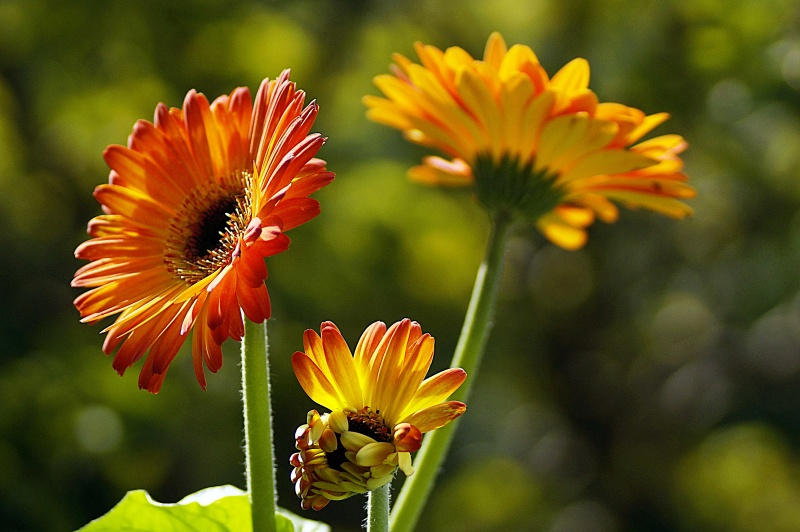
\includegraphics[height=52mm, valign=t]{Immagini/risultati/derodeolifant32584725236.jpg}
    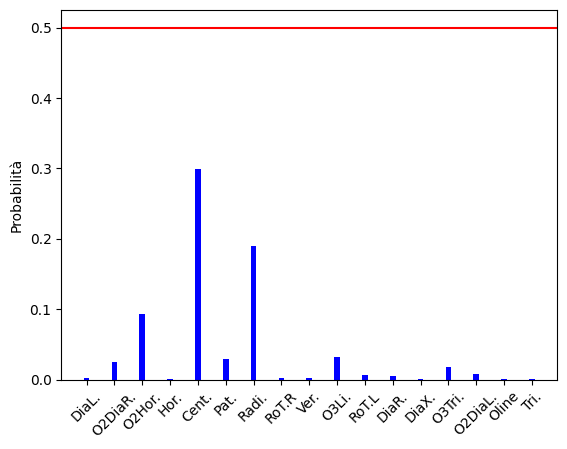
\includegraphics[height=62mm, valign=t]{Immagini/risultati/lodb_1012_prob.png}
    \caption{Predizione con classificatore lineare su LODB, ground truth \textit{O3Tri.}. Il classificatore è molto confuso sulla classe da assegnare, nessuna raggiunge la soglia al di sopra della quale si considerano le predizioni. Questo risultato scarso è in parte dovuto anche all'etichetta assegnata all'immagine. La rete ha delle intuizioni valide: il primo piano di un soggetto viene spesso associato alla classe \textit{Center} nel dataset, prendendo i fiori a coppie si potrebbero considerare come posti in diagonale, il fiore rosso a sinistra è in posizione \textit{RoT.L}, la ripetizione dei petali potrebbe essere visto come \textit{Pattern}, la forma del fiore come \textit{Radi.}. Si notano le limitazioni delle classi introdotte da LODB, di granularità troppo elevata e che spesso si sovrappongono l'una all'altra, nonostante le immagini siano per la maggior parte etichettate con una sola label.}
    \label{fig:lodb_prob}
\end{figure}

\begin{figure}[p]
    \centering
    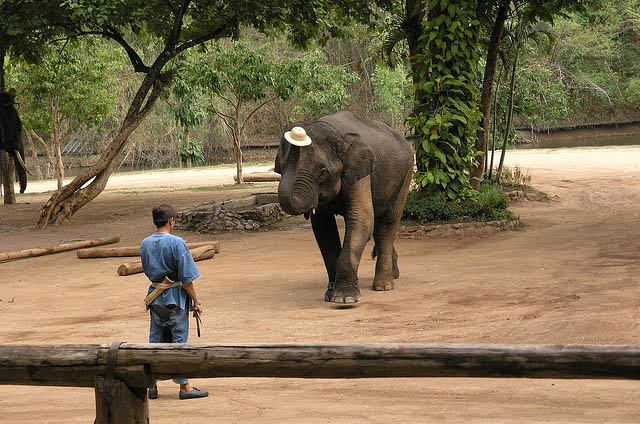
\includegraphics[height=52mm, valign=t]{Immagini/risultati/000000332876_r.jpg}
    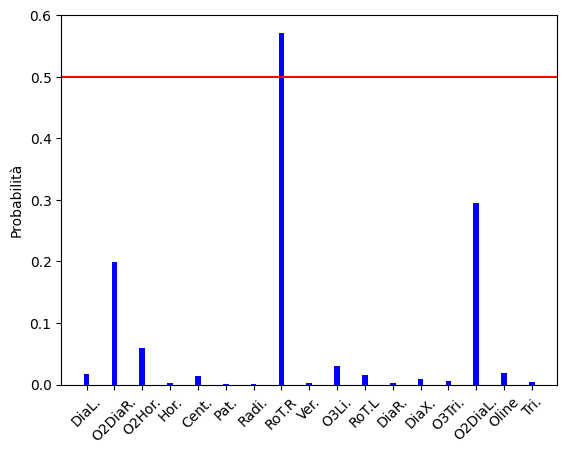
\includegraphics[height=61mm, valign=t]{Immagini/risultati/lodb_130_prob.png}
    \caption{Predizione con classificatore lineare su LODB, ground truth \textit{O2DiaR.}. La rete predice \textit{RoT.R}, sbagliando completamente. \textit{RoT.L} sarebbe potuta essere una buona intuizione, l'uomo si trova all'intersezione degli assi sinistro e inferiore della griglia della regola dei terzi, ma con questa predizione il modello mostra di non aver compreso effettivamente la differenza fra classi \textit{R} e \textit{L}, indicato anche dal fatto che la seconda probabilità più alta sia quella di \textit{O2DiaL}.}
    \label{fig:lodb_prob2}
\end{figure}


\begin{figure}[p]
    \centering
    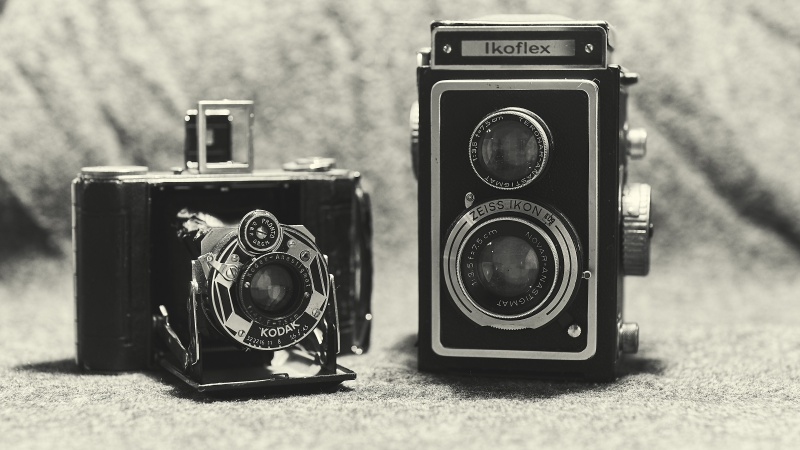
\includegraphics[height=47mm, valign=t]{Immagini/risultati/shcolsson33210898488.jpg}
    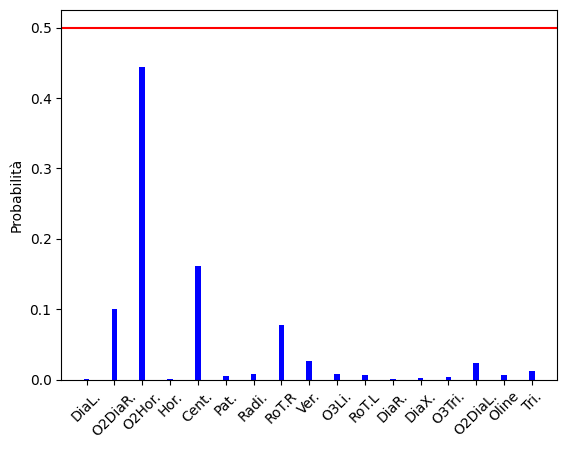
\includegraphics[height=55mm, valign=t]{Immagini/risultati/lodb_154_prob.png}
    \caption{Predizione con classificatore lineare su LODB, ground truth \textit{O2Hor.}. Anche su immagini la cui composizione risulta essere piuttosto chiara all'occhio umano, il modello fatica a riconoscerla e spalma le sue predizioni su diverse classi, facendo fatica a prendere una decisione. }
    \label{fig:lodb_prob3}
\end{figure}